\documentclass[10pt]{article}
\raggedbottom{}
\usepackage[utf8]{inputenc}
\usepackage[papersize={216mm,330mm},tmargin=15mm,bmargin=15mm,lmargin=15mm,rmargin=15mm]{geometry}
\usepackage[english, spanish]{babel}
% \usepackage{fullpage} % changes the margin
\usepackage{graphicx}
\usepackage{enumitem}
\usepackage{chngcntr}
\usepackage{multirow}
\usepackage{parskip}
\usepackage{url}
\usepackage{booktabs} 
\counterwithin{figure}{section}
\renewcommand{\thesection}{\arabic{section}}
\renewcommand{\thesubsection}{\thesection.\arabic{subsection}}
\renewcommand{\baselinestretch}{1.5}
\usepackage{float}
\usepackage{apacite}
\usepackage{multicol}
\bibliographystyle{apacite}
\setlength\belowcaptionskip{10pt}
\linespread{1.5}

\begin{document}

\begin{titlepage}
	\centering
	
\includegraphics[width=0.3\textwidth]{Images/logo_utb.png}\par\vspace{1cm}
	{\scshape\LARGE Universidad Tecnológica de Bolívar \par}
	\vspace{4cm}

	{\scshape\Large FÍSICA ELÉCTRICA \par}
	\vspace{.8cm}

	% chktex-file 8
	{\scshape\Large H1 - C \par}
	\vspace{2.5cm}
	% chktex-file 8
	\slshape {\Large \bfseries{}Informe de Laboratorio No.  \\}
	\vspace{2.5cm}

	\slshape {\itshape{} Mauro González, T00067622 \\}
	\slshape {\itshape{} German De Armas Castaño, T00068765 \\}
	\slshape {\itshape{} Angel Vega Rodriguez, T00068186 \\}
	\slshape {\itshape{} Juan Jose Osorio Ariza, T00067316 \\}
	% \slshape {\itshape{} Juan Eduardo barón, T00065901 \\}
	\vfill
	Revisado Por \\
	Gabriel Hoyos Gomez Casseres\\
	{\large \today\par}
\end{titlepage}

% ----------------------------------------------------------------------|>
\begin{multicols}{2}

	\section{Introducción}

	La ley de Ohm es una ley fundamental de la electricidad que establece una
	relación entre la corriente eléctrica que fluye a través de un conductor,
	la tensión eléctrica aplicada, el voltaje y la resistencia eléctrica del
	propio conductor.

	En el desarrollo de esta practica se busca comprobar si el voltaje es
	proporcional a la corriente que circula por un circuito, en donde se
	considera como única constante a la resistencia que tenga el circuito en sí.

	En esta practica se comprueban algunas de las hipótesis que hay sobre la
	ley de Ohm como lo puede ser el hecho de que sin importar el tipo de
	circuito  con el que se trabaje, este  no tiene ningún tipo de influencia
	sobre la ley de ohm, debido a que en cualquier circuito eléctrico, esta ley
	se aplica a cada componente individual, como resistencias, diodos,
	transistores, entre otros.  De ahí proviene su utilidad en el diseño y
	análisis de circuitos eléctricos

	Durante esta práctica se demuestra la importancia de la ley de Ohm en la
	teoría eléctrica, Para ello mediante la toma de medidas y la realización
	de cálculos, se busca realizar un análisis crítico del comportamiento de
	esta ley, en qué condiciones variaría y como afecta el hecho que hagamos
	el experimento con un material óhmico o no.

	% \newpage

	% ----------------------------------------------------------------------|>
	\section{Objetivos}

	\subsection{Objetivo General}
	
	\begin{itemize}
		\item Explicar y describir la ley de Ohm y su relación con la
		      corriente, el voltaje y la resistencia además de discutir sus
		      limitaciones y sus propiedades.
	\end{itemize}
	
	\subsection{Objetivos específicos}
	
	\begin{itemize}
		\item Reconocer las diferencias entre materiales óhmicos y no óhmicos.
		\item Identificar los valores de resistencia y resistividad.
		\item Comprender la diferencia entre resistencia y resistividad.
	\end{itemize}

	% \newpage

	% ----------------------------------------------------------------------|>

	\section{Marco Teórico}

	% ---------------------------------------------------|>
	\subsection*{Ley de Ohm}

	La Ley de Ohm establece que la corriente eléctrica que fluye a través de un
	circuito es proporcional a la diferencia de potencial eléctrico entre los
	extremos del mismo, y es inversamente proporcional a la resistencia del
	circuito.~\cite{LeyDeOhm}

	% ---------------------------------------------------|>
	\subsection*{Material tipo Ohm}

	Los materiales óhmicos tienen una relación lineal de corriente-diferencia de
	potencial en un largo intervalo de diferencias de potencial aplicadas.
	La pendiente de la curva I v/s $\triangle$V en la región lineal produce un
	valor para 1/R.~\cite{MaterialesOhmicos}

	% ---------------------------------------------------|>
	\subsection*{Deducción a partir de la ley de Ohm}

	La resistencia de un conductor cilíndrico está determinada por su longitud $l$,
	la sección transversal $a$ y la resistividad del material a una temperatura dada.
	La resistencia es directamente proporcional a la longitud $l$ y a la
	resistividad $\rho$, pero inversamente proporcional a su sección transversal.

	$R = p \cdot \frac{l}{a}$

	% ---------------------------------------------------|>
	\subsection*{Factores de los cuales depende la resistencia y resistividad}

	La resistividad de un material óhmico es una propiedad característica que
	depende de su composición y temperatura. Los materiales con resistividad
	cero son considerados conductores ideales, mientras que aquellos con
	resistividad infinita son considerados aislantes ideales. En otras
	palabras, la resistividad de un material es un factor clave en la
	determinación de su capacidad para conducir electricidad.

	% ---------------------------------------------------|>
	\subsection*{Temperatura, resistencia y resistividad}

	La resistividad $\rho$ de un material depende de la estructura molecular y
	atómica, y es dependiente de la temperatura. Para la mayoría de los conductores,
	la resistividad aumenta con el aumento de temperatura.~\cite{KhanAcademy}

\end{multicols}

% ---------------------------------------------------|>
\subsection*{Gráfica de Voltaje vs Corriente}

\begin{figure}[H]
	\begin{center}
		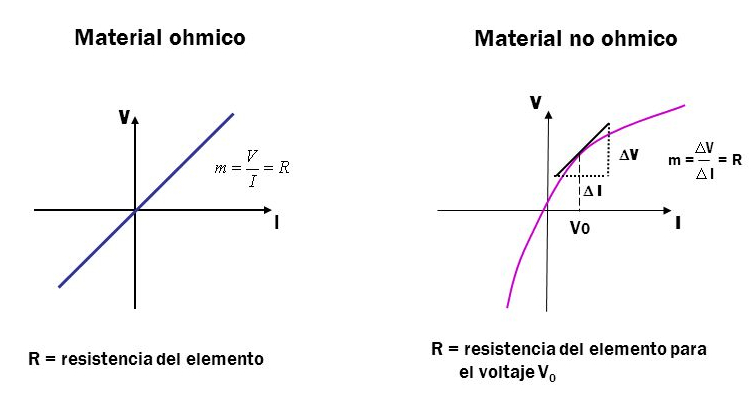
\includegraphics[scale = 0.31]{./Images/VoltajeVsResistencia.jpg}
	\end{center}
\end{figure}


% ----------------------------------------------------------------------|>
\section{Montaje Experimental}

\begin{multicols}{2}
	\begin{itemize}
		\item Alambres resistivos de forma cilíndrica
		\item Calibrador pie de rey
		\item Termómetro
		\item Multímetro digital y multímetro analógico
		\item Fuente de D.C.
		\item Resistor de 500Ω/90mA
		\item Bombillo de 12W/110V
		\item Reóstato de 33Ω/3.1A
	\end{itemize}

	\begin{figure}[H]
		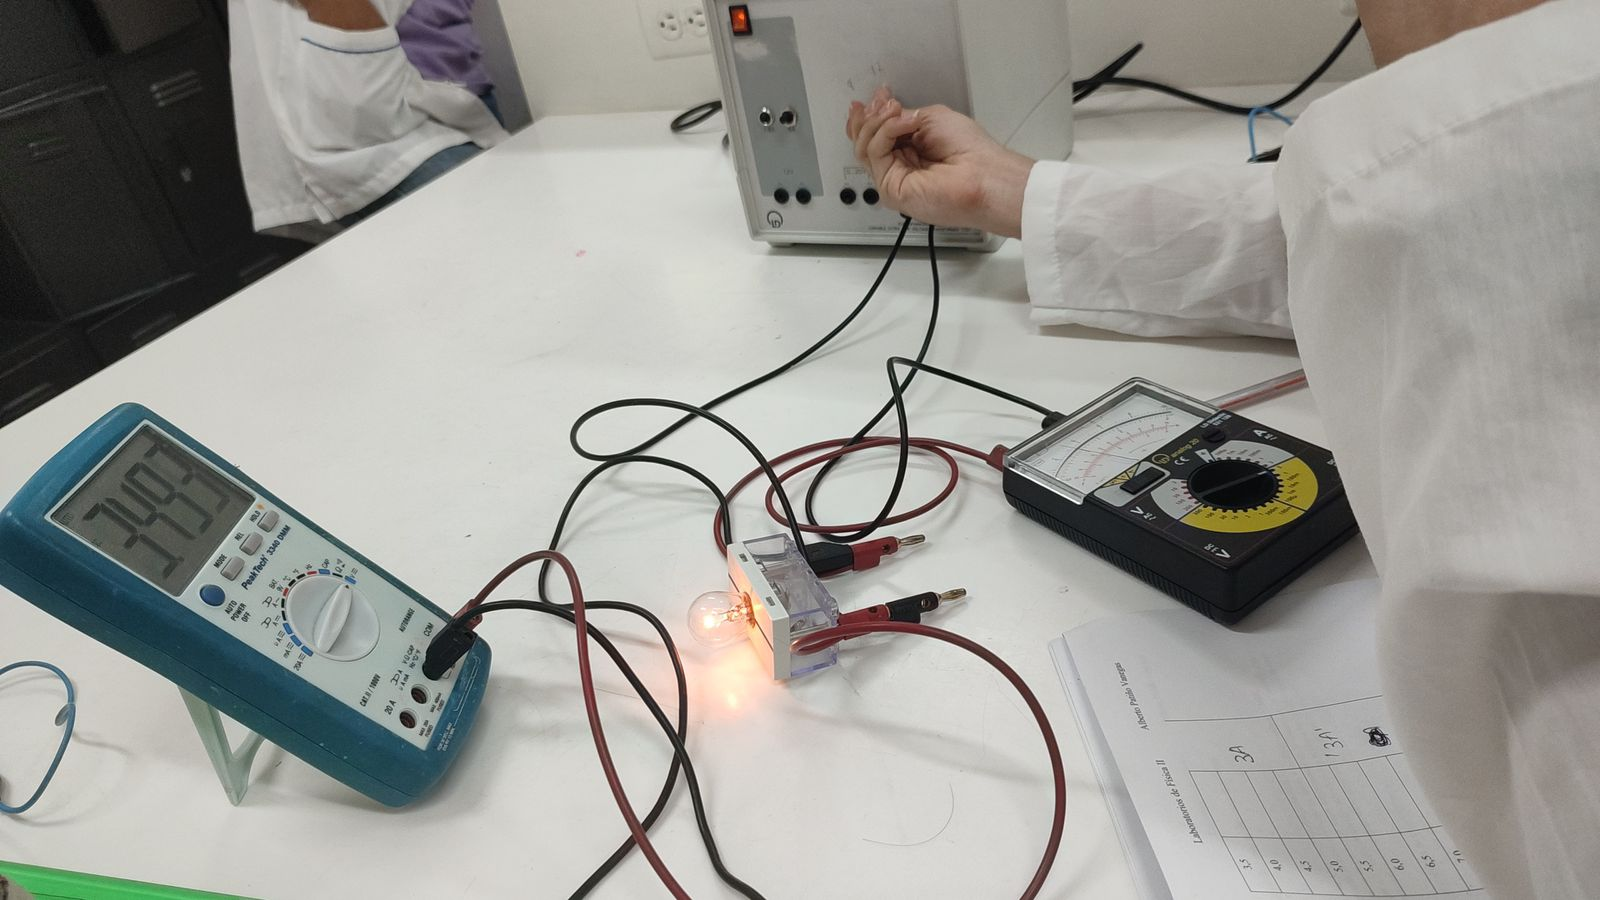
\includegraphics[width=\linewidth]{./Images/ME1.jpeg}
		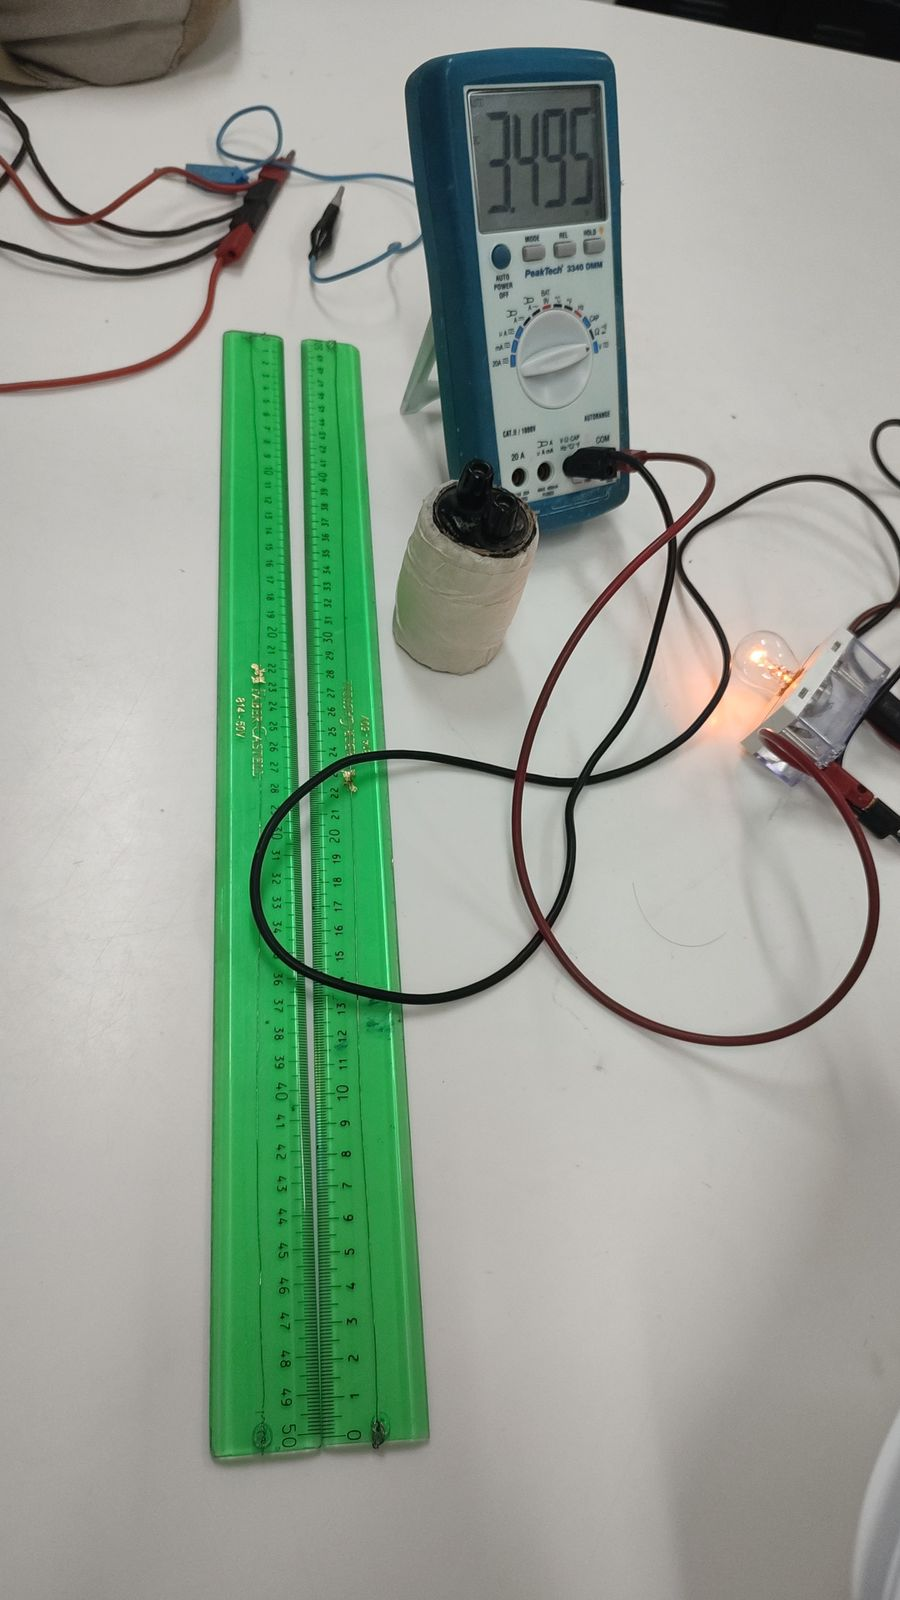
\includegraphics[width=0.5\linewidth]{./Images/ME2.jpeg}
	\end{figure}

\end{multicols}

% ----------------------------------------------------------------------|>
\section{Datos Experimentales}

\begin{table}[H]
	\centering
	\caption{Tabla de valores para resistencia eléctrica}
	% chktex-file 24
	\label{tabla-resistencia 1ra Medicion}
	\begin{tabular}{cccccccc}
		\toprule
		                          & 1                    & 2                                    & 3                  & 4               & 5                  & 6                     & 7                     \\
		\midrule
		R ($\Omega$)              & 0.6                  & 1.6                                  & 1.8                & 2               & 2.4                & 2.8                   & 3.3                   \\
		L/A ($m^{-1}$)            & 0.07                 & 0.14                                 & 0.21               & 0.28            & 0.35               & 0.42                  & 0.49                  \\
		$\rho$ ($\Omega \cdot m$) & $6 \times 10^{-7}$   & $ \times 10^{-7}$                    & $6 \times 10^{-7}$ & $5 \times 10-7$ & $4.8 \times 10^{}$ & $4.67 \times 10^{-7}$ & $4.71 \times 10^{-7}$ \\
		Promedio: $\rho$          & $5.6 \times 10^{-7}$ & \multicolumn{2}{c}{Área Transversal} & $7 \times 10^{-8}$ & Material        & Constantán                                                         \\
		\bottomrule
	\end{tabular}
\end{table}

\begin{table}[H]
	\centering
	\caption{Tabla de valores para resistencia eléctrica}
	% chktex-file 24
	\label{tabla-resistencia 2da Medicion}
	\begin{tabular}{cccccccc}
		\toprule
		                          & 1                     & 2                                    & 3                    & 4                    & 5                    & 6                    & 7                    \\
		\midrule
		R ($\Omega$)              & 1.5                   & 2                                    & 2.8                  & 3.7                  & 4.4                  & 5.2                  & 6                    \\
		L/A ($m^{-1}$)            & 0.07                  & 0.14                                 & 0.21                 & 0.28                 & 0.35                 & 0.42                 & 0.49                 \\
		$\rho$ ($\Omega \cdot m$) & $2.6 \times 10^{-6}$  & $1.7 \times 10^{-6}$                 & $1.6 \times 10^{-6}$ & $1.6 \times 10^{-6}$ & $1.5 \times 10^{-6}$ & $1.5 \times 10^{-6}$ & $1.5 \times 10^{-6}$ \\
		Promedio: $\rho$          & $1.71 \times 10^{-6}$ & \multicolumn{2}{c}{Área Transversal} & $1.2 \times 10^{-7}$ & Material             & Aleación de Fe y Ni                                                \\
		\bottomrule
	\end{tabular}
\end{table}

% \begin{table}[H]
% 	\begin{tabular}{ccc}
% 		\label{tabla-resistor 1ra Medicion}
% 		\toprule
% 		Voltaje $(V)$ & Corriente I $(mA)$ & Escala  \\
% 		\midrule
% 		0.566         & 1                  & $10mA$  \\
% 		1.016         & 2                  &         \\
% 		1.555         & 3                  &         \\
% 		2.032         & 4                  &         \\
% 		2.57          & 5                  &         \\
% 		3.058         & 6                  &         \\
% 		3.56          & 7                  &         \\
% 		4.3           & 8                  &         \\ % chktex-file 44
% 		4.57          & 9                  &         \\
% 		\midrule
% 		4.80          & 10                 & $100mA$ \\
% 		5.09          & 11                 &         \\
% 		5.3           & 12                 &         \\
% 		6.39          & 13                 &         \\
% 		6.80          & 14                 &         \\
% 		\bottomrule
% 	\end{tabular}
% \end{table}

% \begin{table}[H]
% 	\begin{tabular}{ccc}
% 		\label{tabla-resistor 2da Medicion}
% 		\toprule
% 		Voltaje $(V)$ & Corriente I $(mA)$ & Escala \\
% 		\midrule
% 		0.5           & 0.4                & $3mA$  \\
% 		1.0           & 0.5                &        \\
% 		1.5           & 0.6                &        \\
% 		2.0           & 0.7                &        \\
% 		2.5           & 0.8                &        \\
% 		3.0           & 0.85               &        \\
% 		3.5           & 0.9                &        \\
% 		4.0           & 1                  &        \\
% 		4.5           & 1.05               &        \\
% 		5.0           & 1.1                &        \\
% 		5.5           & 1.15               &        \\
% 		6.0           & 1.2                &        \\
% 		6.5           & 1.25               &        \\
% 		7.0           & 1.3                &        \\
% 		7.5           & 1.35               &        \\
% 		8.0           & 1.4                &        \\
% 		8.5           & 1.45               &        \\
% 		9.0           & 1.5                &        \\
% 		9.5           & 1.55               &        \\
% 		10            & 1.6                &        \\
% 		\bottomrule
% 	\end{tabular}
% \end{table}


\begin{multicols}{2}

	\begin{figure}[H]
		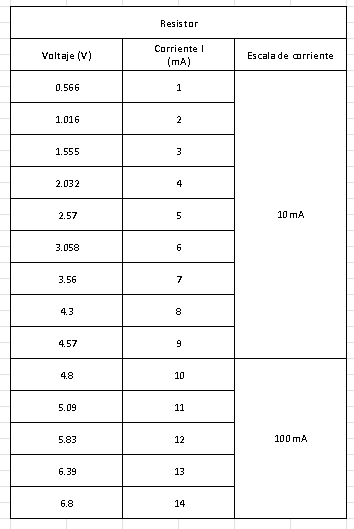
\includegraphics[width = 0.78\linewidth]{./Images/Table1.png}
		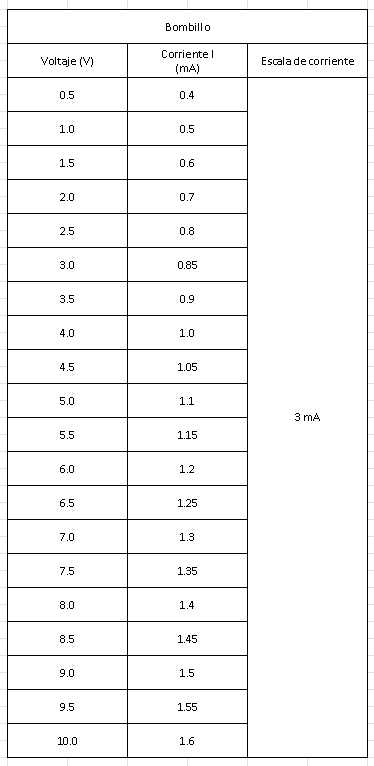
\includegraphics[width = 0.78\linewidth]{./Images/Table2.png}
	\end{figure}

	% \begin{figure}[H]
	% 	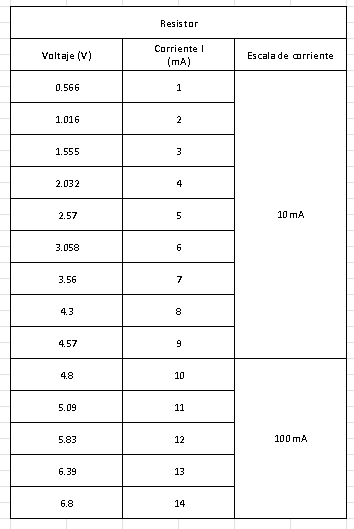
\includegraphics[scale = .50]{./Images/Table1.png}
	% 	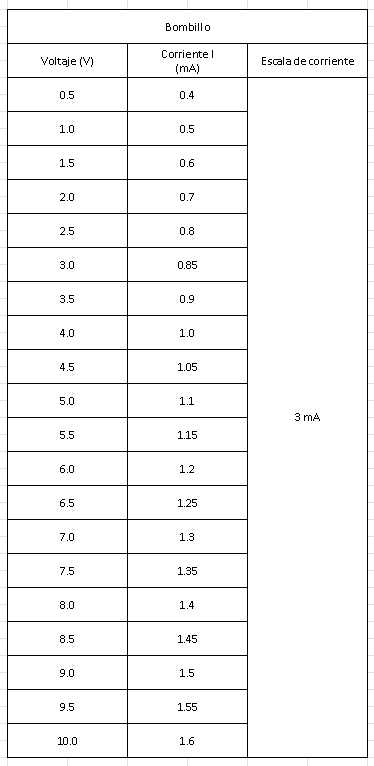
\includegraphics[scale = .55]{./Images/Table2.png}
	% \end{figure}

	% \begin{figure}[H]
	% \end{figure}

	% \end{multicols}

	% ----------------------------------------------------------------------|>
	% \begin{multicols}{2}

	\section{Análisis de datos}

	% ---------------------------------------------------------------------------------------------------------------------------|>
	\subsection{Primera Parte}

	% --------------------------------------------|>
	\subsubsection*{Calcule el área transversal A (en m2)
		de uno de los alambres utilizados}

	\begin{itemize}
		\item Area transversal 1er alambre: $7 \times 10^{-8}$
		\item Area transversal 2do alambre: $1.2 \times 10^{-7}$
	\end{itemize}

	% --------------------------------------------|>
	\subsubsection*{Compare el valor de resistividad encontrado de los diferentes materiales
		registrados en la tabla 4}

	Basado en los resultados, el primer material es Constantán y el segundo es
	una aleación de Fe y Ni.

	% --------------------------------------------|>
	\subsubsection*{¿A qué se debe la diferencia entre el valor de resistividad encontrado y registrado
		en las tablas?}

	La principal distinción se encuentra en la manera en que se debe considerar
	el valor de la resistencia de un material, debido a que en la práctica
	existen variaciones en los intervalos de los valores que se establecen
	para calcularla.

	% --------------------------------------------|>
	\subsubsection*{¿Depende la resistividad de la longitud del alambre?}

	La resistividad es una propiedad intrínseca de los materiales que permite
	comparar su resistencia eléctrica sin considerar la longitud o el área
	transversal del material. Esto se debe a que la resistividad depende de
	factores como la temperatura, la pureza del material y su estructura
	cristalina.~\cite{KhanAcademy}

	% --------------------------------------------|>
	\subsubsection*{¿Depende la resistividad del área transversal del alambre?}

	Basándose en la respuesta anterior, la resistividad no depende
	del area transversal del alambre, ya que esta es una propiedad intrínseca
	de los materiales.~\cite{KhanAcademy}


	% --------------------------------------------|>
	\subsubsection*{¿De qué características del alambre depende la resistividad?}

	La resistividad de un alambre \textit{(y cualquier otro material en general)},
	dependerá del tipo de material del que este hecho, la temperatura,
	la pureza, y la estructura cristalina del material \textit{(Los metales
		que tienen una estructura cristalina mas ordenada suelen tener
		resistividad mas baja)}.~\cite{KhanAcademy}

	% --------------------------------------------|>
	\subsubsection*{¿Depende la resistencia de la longitud del alambre? Explique}

	La resistencia de un alambre depende directamente de su longitud. Esto se
	debe a que la resistencia eléctrica de un conductor está relacionada con
	la distancia que debe recorrer la corriente eléctrica a través del
	conductor. Cuanto más largo sea el alambre, mayor será la distancia que
	debe recorrer la corriente eléctrica y, por lo tanto, mayor será la
	resistencia eléctrica.~\cite{KhanAcademy}

	% --------------------------------------------|>
	\subsubsection*{¿Depende la resistencia del área de la sección transversal del alambre?
		Explique.}

	La resistencia de un alambre depende inversamente de su área de sección
	transversal. Esto se debe a que la sección transversal del alambre está
	directamente relacionada con la cantidad de espacio disponible para que
	los electrones se muevan libremente. Cuanto mayor sea el área de la sección
	transversal del alambre, menor será la resistencia eléctrica que ofrecerá
	al paso de la corriente eléctrica, ya que los electrones tendrán más
	espacio para moverse.%~\cite{KhanAcademy}

	% ---------------------------------------------------------------------------------------------------------------------------|>
	\subsection{Segunda parte}

	% --------------------------------------------|>
	\subsubsection*{Grafique los datos de V vs. I registrados en la tabla 3}

	\begin{figure}[H]
		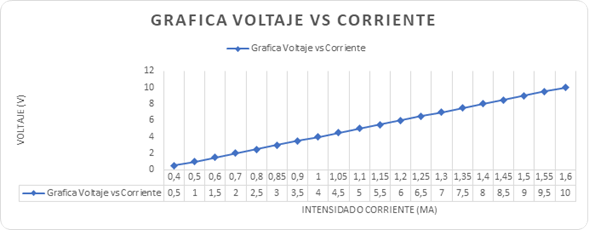
\includegraphics[scale = .55]{./Images/Grafica.png}
	\end{figure}

	% --------------------------------------------|>
	\subsubsection*{Obtenga la ecuación de la curva que mejor se ajusta a los datos mediante el MMC}

	$X = Corriente o Intensidad$	\hfill \break{}
	$Y = Volts$

	\begin{figure}[H]
		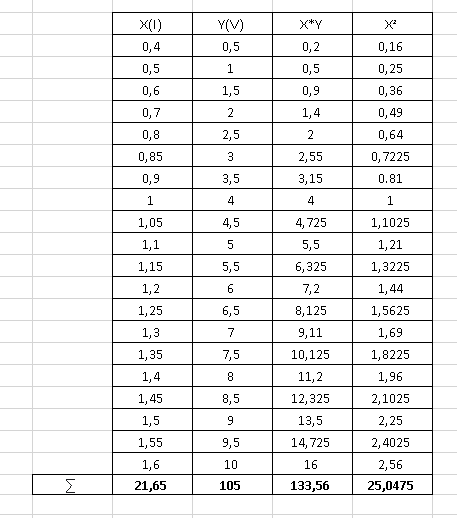
\includegraphics[scale = .5]{./Images/TablaMMC.PNG}
	\end{figure}

	Ecuación de la recta: $y = mx + b$, donde m es la pendiente y b es el punto
	de corte.

	\begin{figure}[H]
		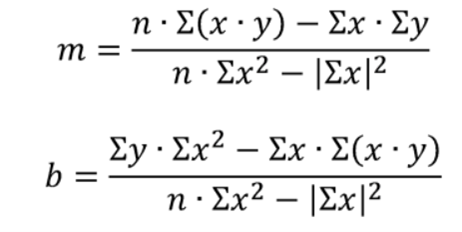
\includegraphics[scale = .5]{./Images/MMC.png}
	\end{figure}

	$m = \frac{20 \cdot (133.56) - (21.65)(105)}{20 \cdot (25.0475) - (468.7225)} = 12.35$

	$b = \frac{105 \cdot 25.0475 - 21.65 \cdot 133.56}{20 \cdot (25.0475) - (468.7225)} = -8.12$

	$y = 12.35x - 8.12$

	% --------------------------------------------|>
	\subsubsection*{Determine a partir de la gráfica el valor experimental de la resistencia del bombillo antes y
		después de conectarlo. Compárelo con el valor medido y explique las posibles causas de error. }

	\begin{figure}[H]
		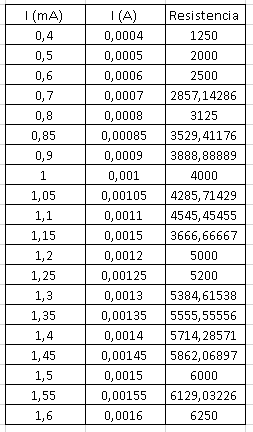
\includegraphics[width = 0.5\linewidth]{./Images/Resistencias.PNG}
	\end{figure}

	Error relativo en la resistencia: $R = \frac{V}{I}$ \hfill \break{}

	$R = 4337.19184 \pm 0,0003$

	Cómo es posible evidenciar teniendo en cuenta los datos y la gráfica, el
	error existente es bajo y se observa en la curva de la gráfica la cuál es
	visualmente una recta que crece linealmente con los datos de voltaje y
	corriente, esto se complementa con la ecuación obtenida con los mínimos
	cuadrados.

	% --------------------------------------------|>
	\subsubsection*{¿Se comporta el resistor como un dispositivo tipo óhmico? Justifique su respuesta. }

	Sí se comparta como un material Óhmico, ya que la curva de la gráfica es
	linealmente creciente y nos demuestra que la relación entre el voltaje y
	la corriente es constante, es decir, son directamente proporcionales.

	Además, en la práctica se observó como la bombilla aumentaba su luminosidad
	a medida que se aumentaba la corriente y el voltaje. Por lo tanto, el bajo
	error relativo en los datos simplemente demuestra la resistencia de la
	bombilla.

\end{multicols}

% ----------------------------------------------------------------------|>
\section{Conclusiones}

% ---------------------------------------|>
\subsection*{Experiencia 1}

En la siguiente experiencia se determinaron aquellos factores que influyen
directamente en la resistividad de un material (Ya sea o no Óhmico) como lo
es la temperatura, la pureza del material, estructura cristalina, entre otras
cosas; esto quiere decir que aquellos factores como el área transversal no
interfieren en esta; sin embargo, existen otros que, aunque no interfieren
con la resistividad y lo hacen con la resistencia como lo es la longitud,
con la cual tiene una relación directa debido a la distancia que recorre
la corriente eléctrica en el material.

% ---------------------------------------|>
\subsection*{Experiencia 2}

Se pudo hacer uso de método muy eficientes como el de los mínimos cuadrados
a la hora de realizar comparaciones en las gráficas entre los valores
obtenidos y los esperados, de esta forma se estimaba la resistividad 
del material principalmente visto al momento de obtener el calculo 
de la pendiente.

% ---------------------------------------|>
\subsection*{Experiencia 3}

En esta experiencia se pudo determinar el comportamiento que tienen los 
materiales óhmicos en comparación de los no óhmicos, se evidenció como 
se mantenía una resistencia lineal entre el voltaje y la corriente para 
brindarle un flujo estable a la bombilla, la cuál aumentaba su 
luminosidad progresivamente a medida que aumentaban los factores 
influyentes (voltaje y corriente). Gracias al método de mínimos 
cuadrados fue posible realizar comparaciones entre los gráficos 
y realizar las respectivas observaciones. 

\bibliography{./Bibliography/bibliography.bib}

\end{document}